% Chapter 7
\chapter{Experimentálne výsledky.}\label{Chapter7}
\lhead{Kapitola 7. \emph{Experimentálne výsledky}}

Záverečný experiment bol uskutočnený na štruktúrach MOS s nehomogénnym
hĺbkovým profilom dotujúcich prímesí, ktorý bol vytvorený procesom
iónovej implantácie s rôznymi dávkami v monokryštále kremíka typu N s
orientáciou [100].

Pred technologickým spracovaním bola otestovaná homogenita
špecifického odporu použitých kremíkových dosiek pomocou zariadenia
Prometrix OmniMap RS35, ktoré využíva štvorbodovú metódu pre určenie
povrchového špecifického odporu. V tabuľke~\ref{tab:7.1} sú uvedené
stredné hodnoty špecifického odporu $\overline\rho$ a smerodajnej
odchýlky $\delta\rho$ vyjadrenej absolútnou a relatívnou hodnotou.

\begin{table}[h!]\centering
  \begin{minipage}[c]{\myfiguresize}
    \begin{center}
      \begin{tabular}{c c c c c c c c}
        č. & $\overline\rho[\Omega cm]$ & $\delta\rho[\Omega cm]$ & $\delta\rho[\%]$ &
        č. & $\overline\rho[\Omega cm]$ & $\delta\rho[\Omega cm]$ & $\delta\rho[\%]$\\
        \hline% chktex-file 44
        1  & 4.3319 & 0.1223 & 2.822 & 11 & 4.5706 & 0.1658 & 3.627\\
        2  & 4.2733 & 0.1204 & 2.817 & 12 & 4.4762 & 0.1860 & 4.155\\
        3  & 5.1040 & 0.3405 & 6.671 & 13 & 4.3332 & 0.1265 & 2.290\\
        4  & 4.6276 & 0.2080 & 4.494 & 14 & 4.8422 & 0.3573 & 7.380\\
        5  & 4.7697 & 0.1824 & 3.824 & 15 & 4.5917 & 0.1741 & 3.791\\
        6  & 4.8007 & 0.2340 & 4.873 & 16 & 4.8134 & 0.2590 & 5.380\\
        7  & 4.2500 & 0.1436 & 3.378 & 17 & 4.4025 & 0.1527 & 3.468\\
        8  & 4.8259 & 0.3163 & 6.554 & 18 & 4.3591 & 0.1290 & 2.960\\
        9  & 4.2853 & 0.1418 & 3.308 & 19 & 4.3877 & 0.1349 & 3.074\\
        10 & 4.2954 & 0.1113 & 2.592 & 20 & 4.5416 & 0.1618 & 3.563\\
      \end{tabular}
    \end{center}
    \caption[Stredná hodnota a smerodajná odchýlka špecifického odporu
      testovaných kremíkových dosiek pred technologickým
      spracovaním]{Stredná hodnota a smerodajná odchýlka špecifického
      odporu testovaných kremíkových dosiek pred technologickým
      spracovaním.}\label{tab:7.1}
  \end{minipage}
\end{table}

Zariadenie Prometrix OmniMap RS35 zmeralo pomocou krokovacieho
zariadenia hodnotu špecifického odporu v 81 bodoch každej dosky. Na
obrázku~\ref{fig:7.1} a obrázku~\ref{fig:7.2} uvádzame grafické
znázornenie rozloženia špecifického odporu, ktoré je taktiež výstupom
merania uvedeného zariadenia. Body, v ktorých bol zmeraný špecifický
odpor sú na obrázku~\ref{fig:7.1} vyznačené znakmi $+$, alebo $-$
podľa toho, či hodnota špecifického odporu v tomto bode ležala nad,
alebo pod strednou hodnotou, ktorá je znázornená hrubšou čiarou.
Predstavu o kvantitatívnom rozložení špecifického odporu si možno
urobiť z trojdimenzionálneho obrázku~\ref{fig:7.2}.

Postup hlavných technologických operácií vytvorenia štruktúr MOS na
uvedených substrátoch bol následovný

\begin{itemize}
\item vytvorenie hradlového oxidu s hrúbkou $100 \nu m$
\item implantácia $P^{31}$ s energiou $120 keV$ a dávkami 0.6, 1.0,
  2.0, 4.0, 5.0, 6.0, 7.0, 8.0, 20.0, 60.0 $\times 10^{15} m^{-2}$ pod
  uhlom $7\degree$
\item aktivácia pri teplote $1050 \degree C$ s časovým priebehom: 15
  min.\ nábeh, 30 min.\ aktivácia, 40 min.\ chladenie
\item naparenie Al na obe strany kremíkovej dosky
\item litografický proces vytvorenia CV masky
\item sintrovanie Al FG pri teplote $460 \degree C$ počas 20 min.
\end{itemize}

Uvedeným spôsobom bolo pripravených 20 kremíkových dosiek o priemere 4
palce, vždy dve s rovnakou dávkou implantácie.  V procese zberu dát
bolo na každej kremíkovej doske testovaných 304 štruktúr, pričom
plocha jednej štruktúry bola $0.81 \times 10^{-6} m^{-2}$. Na
obrázku~\ref{fig:7.3} sú znázornené priebehy koncentračných profilov
dotujúcich prímesi pre jednotlivé dávky implantácie. Znázornené
priebehy predstavujú strednú hodnotu cez všetky závislosti $N(x)$,
ktoré boli určené na testovanej doske. Z každej dávky je na
obrázku~\ref{fig:7.3} zobrazená len jedna kremíková doska.

\newpage
\begin{figure}[h!]\centering
  \begin{minipage}[c]{\myfiguresize}
    \begin{center}
      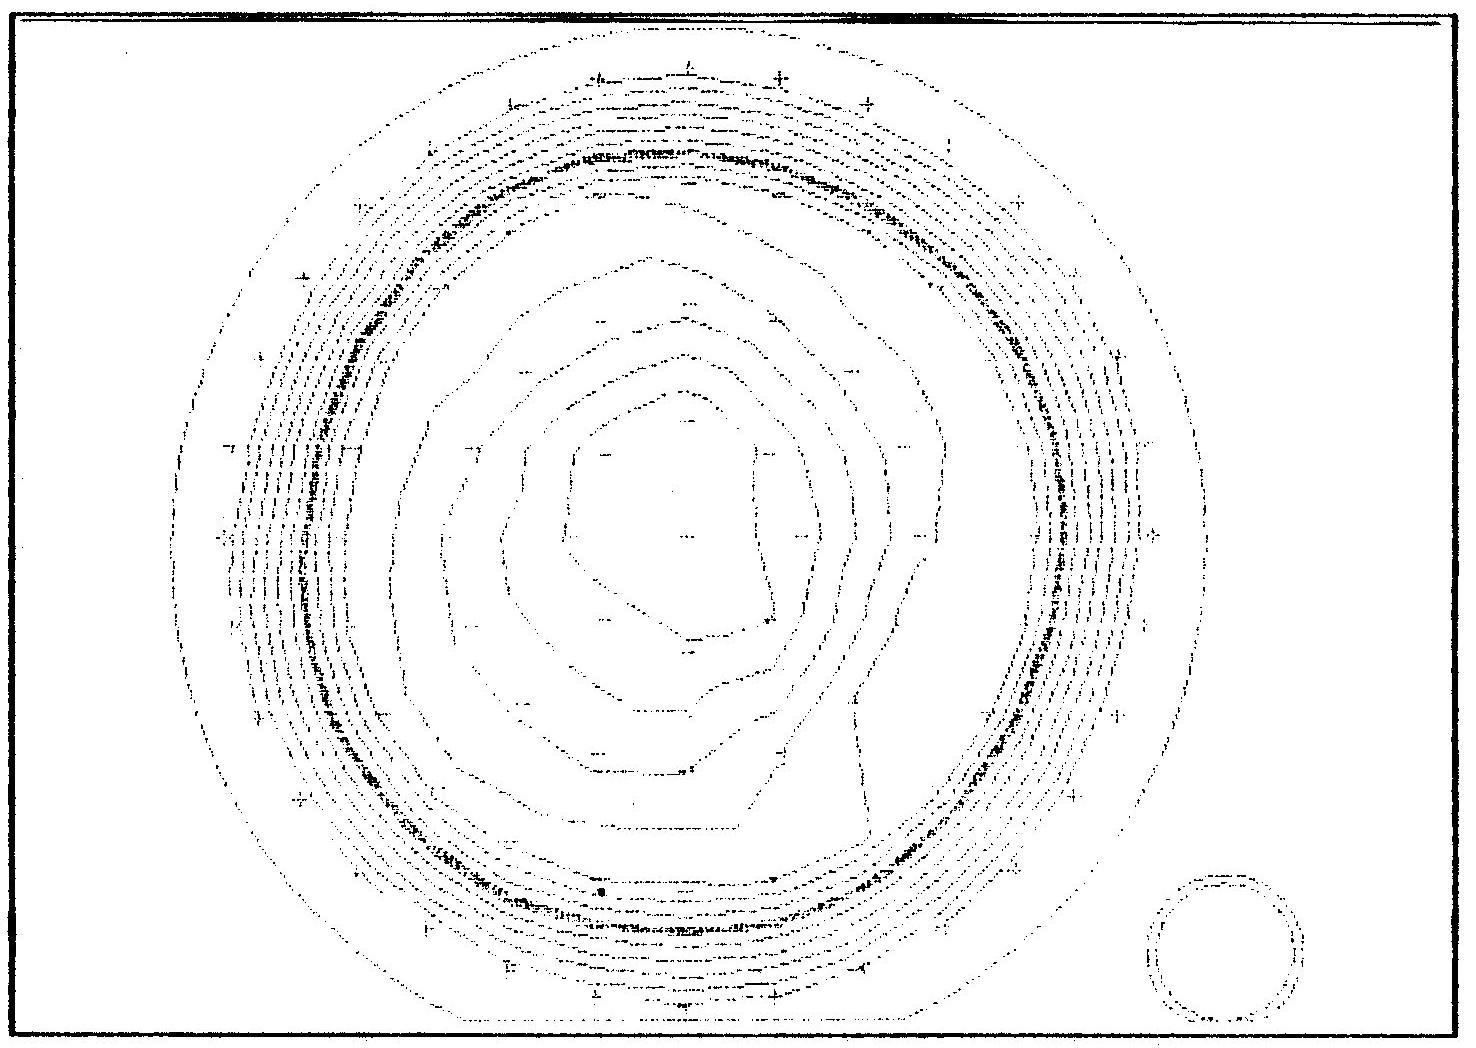
\includegraphics{Figures/fig-7-1.eps}% chktex-file 8
    \end{center}
    \caption[Plošné rozloženie povrchového špecifického odporu
      kremíkovej dosky č.16]{Plošné rozloženie povrchového
      špecifického odporu kremíkovej dosky č.16.}\label{fig:7.1}
  \end{minipage}
\end{figure}

\begin{figure}[h!]\centering
  \begin{minipage}[c]{\myfiguresize}
    \begin{center}
      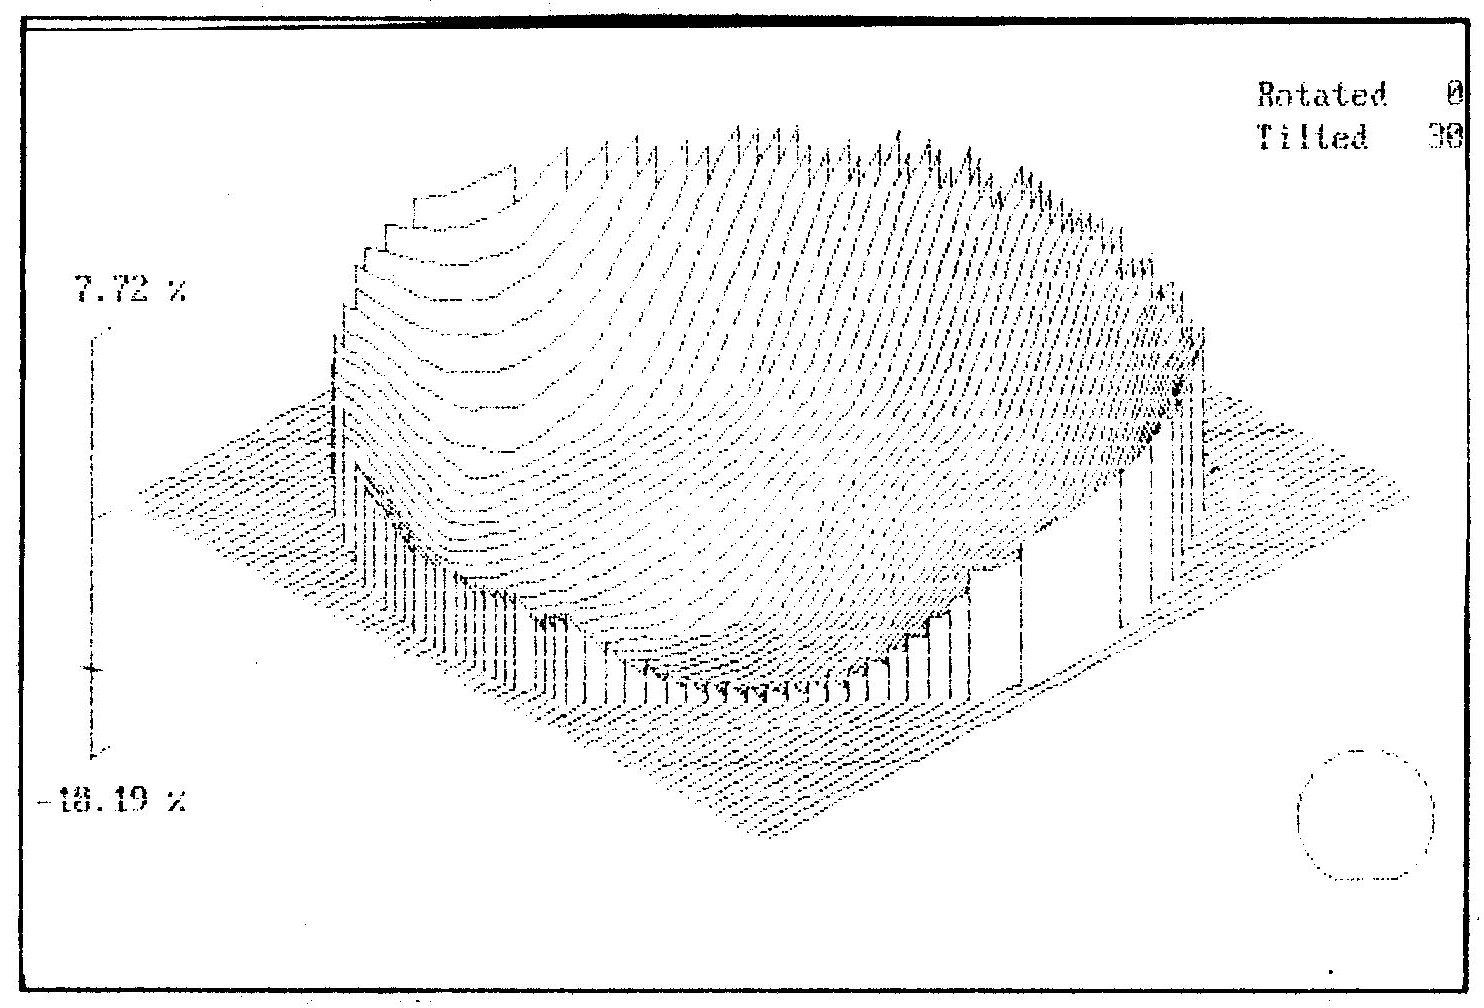
\includegraphics{Figures/fig-7-2.eps}
    \end{center}
    \caption[Plošné rozloženie povrchového špecifického odporu
      kremíkovej dosky č.16]{Plošné rozloženie povrchového
      špecifického odporu kremíkovej dosky č.16.}\label{fig:7.2}
  \end{minipage}
\end{figure}

\newpage
\begin{figure}[h!]\centering
  \begin{minipage}[c]{\myfiguresize}
    \begin{center}
      % GNUPLOT: LaTeX picture with Postscript
\begingroup
  \makeatletter
  \providecommand\color[2][]{%
    \GenericError{(gnuplot) \space\space\space\@spaces}{%
      Package color not loaded in conjunction with
      terminal option `colourtext'%
    }{See the gnuplot documentation for explanation.%
    }{Either use 'blacktext' in gnuplot or load the package
      color.sty in LaTeX.}%
    \renewcommand\color[2][]{}%
  }%
  \providecommand\includegraphics[2][]{%
    \GenericError{(gnuplot) \space\space\space\@spaces}{%
      Package graphicx or graphics not loaded%
    }{See the gnuplot documentation for explanation.%
    }{The gnuplot epslatex terminal needs graphicx.sty or graphics.sty.}%
    \renewcommand\includegraphics[2][]{}%
  }%
  \providecommand\rotatebox[2]{#2}%
  \@ifundefined{ifGPcolor}{%
    \newif\ifGPcolor
    \GPcolortrue
  }{}%
  \@ifundefined{ifGPblacktext}{%
    \newif\ifGPblacktext
    \GPblacktexttrue
  }{}%
  % define a \g@addto@macro without @ in the name:
  \let\gplgaddtomacro\g@addto@macro
  % define empty templates for all commands taking text:
  \gdef\gplbacktext{}%
  \gdef\gplfronttext{}%
  \makeatother
  \ifGPblacktext
    % no textcolor at all
    \def\colorrgb#1{}%
    \def\colorgray#1{}%
  \else
    % gray or color?
    \ifGPcolor
      \def\colorrgb#1{\color[rgb]{#1}}%
      \def\colorgray#1{\color[gray]{#1}}%
      \expandafter\def\csname LTw\endcsname{\color{white}}%
      \expandafter\def\csname LTb\endcsname{\color{black}}%
      \expandafter\def\csname LTa\endcsname{\color{black}}%
      \expandafter\def\csname LT0\endcsname{\color[rgb]{1,0,0}}%
      \expandafter\def\csname LT1\endcsname{\color[rgb]{0,1,0}}%
      \expandafter\def\csname LT2\endcsname{\color[rgb]{0,0,1}}%
      \expandafter\def\csname LT3\endcsname{\color[rgb]{1,0,1}}%
      \expandafter\def\csname LT4\endcsname{\color[rgb]{0,1,1}}%
      \expandafter\def\csname LT5\endcsname{\color[rgb]{1,1,0}}%
      \expandafter\def\csname LT6\endcsname{\color[rgb]{0,0,0}}%
      \expandafter\def\csname LT7\endcsname{\color[rgb]{1,0.3,0}}%
      \expandafter\def\csname LT8\endcsname{\color[rgb]{0.5,0.5,0.5}}%
    \else
      % gray
      \def\colorrgb#1{\color{black}}%
      \def\colorgray#1{\color[gray]{#1}}%
      \expandafter\def\csname LTw\endcsname{\color{white}}%
      \expandafter\def\csname LTb\endcsname{\color{black}}%
      \expandafter\def\csname LTa\endcsname{\color{black}}%
      \expandafter\def\csname LT0\endcsname{\color{black}}%
      \expandafter\def\csname LT1\endcsname{\color{black}}%
      \expandafter\def\csname LT2\endcsname{\color{black}}%
      \expandafter\def\csname LT3\endcsname{\color{black}}%
      \expandafter\def\csname LT4\endcsname{\color{black}}%
      \expandafter\def\csname LT5\endcsname{\color{black}}%
      \expandafter\def\csname LT6\endcsname{\color{black}}%
      \expandafter\def\csname LT7\endcsname{\color{black}}%
      \expandafter\def\csname LT8\endcsname{\color{black}}%
    \fi
  \fi
    \setlength{\unitlength}{0.0500bp}%
    \ifx\gptboxheight\undefined%
      \newlength{\gptboxheight}%
      \newlength{\gptboxwidth}%
      \newsavebox{\gptboxtext}%
    \fi%
    \setlength{\fboxrule}{0.5pt}%
    \setlength{\fboxsep}{1pt}%
\begin{picture}(7920.00,5616.00)%
    \gplgaddtomacro\gplbacktext{%
      \csname LTb\endcsname%%
      \put(1100,640){\makebox(0,0)[r]{\strut{}$1\times10^{21}$}}%
      \put(1100,2261){\makebox(0,0)[r]{\strut{}$1\times10^{22}$}}%
      \put(1100,3882){\makebox(0,0)[r]{\strut{}$1\times10^{23}$}}%
      \put(1220,440){\makebox(0,0){\strut{}$0$}}%
      \put(2012,440){\makebox(0,0){\strut{}$0.1$}}%
      \put(2805,440){\makebox(0,0){\strut{}$0.2$}}%
      \put(3597,440){\makebox(0,0){\strut{}$0.3$}}%
      \put(4390,440){\makebox(0,0){\strut{}$0.4$}}%
      \put(5182,440){\makebox(0,0){\strut{}$0.5$}}%
      \put(5974,440){\makebox(0,0){\strut{}$0.6$}}%
      \put(6767,440){\makebox(0,0){\strut{}$0.7$}}%
      \put(7559,440){\makebox(0,0){\strut{}$0.8$}}%
    }%
    \gplgaddtomacro\gplfronttext{%
      \csname LTb\endcsname%%
      \put(190,2827){\rotatebox{-270}{\makebox(0,0){\strut{}Koncentrácia $[{m}^{-3}]$}}}%
      \put(4389,140){\makebox(0,0){\strut{}Hĺbka $[\mu{m}]$}}%
      \put(4389,5315){\makebox(0,0){\strut{}Kocentrácia dopantov}}%
    }%
    \gplbacktext
    \put(0,0){\includegraphics{/export/scratch/vbotka-thesis/Plot/Figures/fig-7-3-sk}}%
    \gplfronttext
  \end{picture}%
\endgroup

    \end{center}
    \caption[Hĺbkový profil dotujúcich prímesí]{Hĺbkový profil
      dotujúcich prímesí v podpovrchovej oblasti polovodiča vytvorený
      iónovou implantáciou s dávkami $0.6, 1.0, 2.0, 4.0, 5.0, 6.0,
      7.0, 8.0, 20.0, 60.0 \times 10^{15} m^{-2}$. Zobrazené priebehy
      $N(x)$ predstavujú strednú hodnotu z priebehov, nameraných na
      304 štruktúrach MOS každej kremíkovej dosky.}\label{fig:7.3}
  \end{minipage}
\end{figure}
% OBR27.BIT

\newpage
\begin{figure}[h!]
  \begin{minipage}[c]{\myfiguresize}
    \begin{center}
      % GNUPLOT: LaTeX picture with Postscript
\begingroup
  \makeatletter
  \providecommand\color[2][]{%
    \GenericError{(gnuplot) \space\space\space\@spaces}{%
      Package color not loaded in conjunction with
      terminal option `colourtext'%
    }{See the gnuplot documentation for explanation.%
    }{Either use 'blacktext' in gnuplot or load the package
      color.sty in LaTeX.}%
    \renewcommand\color[2][]{}%
  }%
  \providecommand\includegraphics[2][]{%
    \GenericError{(gnuplot) \space\space\space\@spaces}{%
      Package graphicx or graphics not loaded%
    }{See the gnuplot documentation for explanation.%
    }{The gnuplot epslatex terminal needs graphicx.sty or graphics.sty.}%
    \renewcommand\includegraphics[2][]{}%
  }%
  \providecommand\rotatebox[2]{#2}%
  \@ifundefined{ifGPcolor}{%
    \newif\ifGPcolor
    \GPcolortrue
  }{}%
  \@ifundefined{ifGPblacktext}{%
    \newif\ifGPblacktext
    \GPblacktexttrue
  }{}%
  % define a \g@addto@macro without @ in the name:
  \let\gplgaddtomacro\g@addto@macro
  % define empty templates for all commands taking text:
  \gdef\gplbacktext{}%
  \gdef\gplfronttext{}%
  \makeatother
  \ifGPblacktext
    % no textcolor at all
    \def\colorrgb#1{}%
    \def\colorgray#1{}%
  \else
    % gray or color?
    \ifGPcolor
      \def\colorrgb#1{\color[rgb]{#1}}%
      \def\colorgray#1{\color[gray]{#1}}%
      \expandafter\def\csname LTw\endcsname{\color{white}}%
      \expandafter\def\csname LTb\endcsname{\color{black}}%
      \expandafter\def\csname LTa\endcsname{\color{black}}%
      \expandafter\def\csname LT0\endcsname{\color[rgb]{1,0,0}}%
      \expandafter\def\csname LT1\endcsname{\color[rgb]{0,1,0}}%
      \expandafter\def\csname LT2\endcsname{\color[rgb]{0,0,1}}%
      \expandafter\def\csname LT3\endcsname{\color[rgb]{1,0,1}}%
      \expandafter\def\csname LT4\endcsname{\color[rgb]{0,1,1}}%
      \expandafter\def\csname LT5\endcsname{\color[rgb]{1,1,0}}%
      \expandafter\def\csname LT6\endcsname{\color[rgb]{0,0,0}}%
      \expandafter\def\csname LT7\endcsname{\color[rgb]{1,0.3,0}}%
      \expandafter\def\csname LT8\endcsname{\color[rgb]{0.5,0.5,0.5}}%
    \else
      % gray
      \def\colorrgb#1{\color{black}}%
      \def\colorgray#1{\color[gray]{#1}}%
      \expandafter\def\csname LTw\endcsname{\color{white}}%
      \expandafter\def\csname LTb\endcsname{\color{black}}%
      \expandafter\def\csname LTa\endcsname{\color{black}}%
      \expandafter\def\csname LT0\endcsname{\color{black}}%
      \expandafter\def\csname LT1\endcsname{\color{black}}%
      \expandafter\def\csname LT2\endcsname{\color{black}}%
      \expandafter\def\csname LT3\endcsname{\color{black}}%
      \expandafter\def\csname LT4\endcsname{\color{black}}%
      \expandafter\def\csname LT5\endcsname{\color{black}}%
      \expandafter\def\csname LT6\endcsname{\color{black}}%
      \expandafter\def\csname LT7\endcsname{\color{black}}%
      \expandafter\def\csname LT8\endcsname{\color{black}}%
    \fi
  \fi
    \setlength{\unitlength}{0.0500bp}%
    \ifx\gptboxheight\undefined%
      \newlength{\gptboxheight}%
      \newlength{\gptboxwidth}%
      \newsavebox{\gptboxtext}%
    \fi%
    \setlength{\fboxrule}{0.5pt}%
    \setlength{\fboxsep}{1pt}%
\begin{picture}(7920.00,5616.00)%
    \gplgaddtomacro\gplbacktext{%
      \csname LTb\endcsname%%
      \put(740,640){\makebox(0,0)[r]{\strut{}$0.1$}}%
      \put(740,2215){\makebox(0,0)[r]{\strut{}$1$}}%
      \put(740,3790){\makebox(0,0)[r]{\strut{}$10$}}%
      \put(860,440){\makebox(0,0){\strut{}$0.1$}}%
      \put(3168,440){\makebox(0,0){\strut{}$1$}}%
      \put(5475,440){\makebox(0,0){\strut{}$10$}}%
    }%
    \gplgaddtomacro\gplfronttext{%
      \csname LTb\endcsname%%
      \put(190,2827){\rotatebox{-270}{\makebox(0,0){\strut{}Aktivované ióny ${10}^{15}[{m}^{-2}]$}}}%
      \put(4209,140){\makebox(0,0){\strut{}Implantačná dávka $D_{i}{10}^{15}[{m}^{-2}]$}}%
      \put(4209,5315){\makebox(0,0){\strut{}Aktivácia dopantov}}%
    }%
    \gplgaddtomacro\gplbacktext{%
      \csname LTb\endcsname%%
      \put(740,640){\makebox(0,0)[r]{\strut{}$0.1$}}%
      \put(740,2215){\makebox(0,0)[r]{\strut{}$1$}}%
      \put(740,3790){\makebox(0,0)[r]{\strut{}$10$}}%
      \put(860,440){\makebox(0,0){\strut{}$0.1$}}%
      \put(3168,440){\makebox(0,0){\strut{}$1$}}%
      \put(5475,440){\makebox(0,0){\strut{}$10$}}%
    }%
    \gplgaddtomacro\gplfronttext{%
      \csname LTb\endcsname%%
      \put(190,2827){\rotatebox{-270}{\makebox(0,0){\strut{}Aktivované ióny ${10}^{15}[{m}^{-2}]$}}}%
      \put(4209,140){\makebox(0,0){\strut{}Implantačná dávka $D_{i}{10}^{15}[{m}^{-2}]$}}%
      \put(4209,5315){\makebox(0,0){\strut{}Aktivácia dopantov}}%
    }%
    \gplbacktext
    \put(0,0){\includegraphics{/export/scratch/vbotka-thesis/Plot/Figures/fig-7-4-sk}}%
    \gplfronttext
  \end{picture}%
\endgroup

    \end{center}
    \caption[Závislosť strednej hodnoty
      $\overline{D}=E(\int(N(x)-N_{b})dx)$ od dávky implantovaných
      iónov $D_{i}$]{Závislosť strednej hodnoty
      $\overline{D}=E(\int(N(x)-N_{b})dx)$ od dávky implantovaných
      iónov $D_{i}$. Dáta z Tabuľky~\ref{tab:7.2}.}\label{fig:7.4}
  \end{minipage}
\end{figure}
%OBR29.BIT

Tabuľka~\ref{tab:7.2} obsahuje číselné hodnoty implantačnej dávky
zadané v procese implantácie $D_{i}$, strednú hodnotu $\overline D$ a
smerodajnú odchýlku $\delta D$ dávok vypočítaných postupom uvedeným v
časti~\ref{sec:6.1}.

\begin{table}[h!]\centering
  \begin{minipage}[c]{\myfiguresize}
    \begin{center}
      \begin{tabular}{c c c c}
        \hline
        č. & ${D_{i}}{10}^{15}[m^{-2}]$ & $\overline{D}{10}^{15}[m^{-2}]$ & $\delta{D}{10}^{15}[m^{-2}]$\\
        \hline
         1 &  0.6 &  0.39 &  0.02\\
         3 &  1.0 &  0.59 &  0.08\\
         5 &  2.0 &  1.20 &  0.06\\
         7 &  4.0 &  2.67 &  0.09\\
         9 &  5.0 &  3.40 &  0.13\\
        11 &  6.0 &  4.07 &  0.13\\
        13 &  7.0 &  4.72 &  0.14\\
        15 &  8.0 &  5.49 &  0.09\\
        17 & 20.0 & 14.41 &  0.35\\
        19 & 60.0 & 42.63 &  0.21\\
        \hline
      \end{tabular}
    \end{center}
    \caption[Dávky implantácie $D_{i}$]{Dávka implantácie $D_{i}$,
      vypočítaná stredná hodnota dávky implantovaných a aktivovaných
      iónov v polovodiči $\overline D$ a jej smerodajná odchýlka
      $\delta D$ na kremíkovej doske.}\label{tab:7.2}
  \end{minipage}
\end{table}

Pre kontrolu reprodukovateľnosti procesu implantácie boli zmerané
koncentračné profily na ďalších 3 kremíkových doskách.  V
tabuľke~\ref{tab:7.3} sa nachádzajú hodnoty dávok implantácie pre tri
dvojice kremíkových dosiek, ktoré boli implantované s tou istou
dávkou.

\begin{table}[h!]\centering
  \begin{minipage}[c]{\myfiguresize}
    \begin{center}
      \begin{tabular}{c c c c}
        \hline
        č. & $D_{i} 10^{15} [m^{-2}]$ & $\overline D 10^{15} [m^{-2}]$ & $\delta D 10^{15} [m^{-2}]$\\
        \hline
         9 & 5.0 & 3.40 & 0.13\\
        10 & 5.0 & 3.56 & 0.06\\
        11 & 6.0 & 4.07 & 0.13\\
        12 & 6.0 & 4.03 & 0.12\\
        15 & 8.0 & 5.49 & 0.09\\
        16 & 8.0 & 5.46 & 0.08\\
        \hline
      \end{tabular}
    \end{center}
    \caption[Dávka implantácie $D_{i}$]{Dávka implantácie $D_{i}$,
      vypočítaná stredná hodnota dávky implantovaných a aktivovaných
      iónov v polovodiči $\overline D$ a jej smerodajná odchýlka
      $\delta D$ na kremíkovej doske.}\label{tab:7.3}
  \end{minipage}
\end{table}

Ako je zrejmé z tabuľky~\ref{tab:7.2} a~\ref{tab:7.3}, vypočítaná
implantačná dávka je vždy menšia ako dávka zadaná v procese
implantácie. To je spôsobené jednako tým, že čas implantovaných iónov
je zachytená v oxidovej vrstve a jednako neúplnou aktiváciou
implantovaných iónov v polovodiči. Aby sme určili závislosť medzi
zadanou a vypočítanou dávkou, vypočítali sme lineárnou regresiou
koeficient $b$ vzťahu

\begin{equation}\label{eq:7.1}
  \overline D = bD_{i}
\end{equation}

ktorý mal hodnotu $b = 0.71$ a zároveň sme zobrazili závislosť
$\overline D = f(D_{i})$ na obrázku~\ref{fig:7.4}. Tým sme zistili, že
z pôvodnej dávky, ktorá bola implantovaná sa stalo elektricky
aktívnymi 71\% implantovaných iónov. Aby sme určili stupeň závislosti
medzi implantovanou dávkou a množstvom elektricky aktívnych prímesí v
polovodiči, ktoré boli implantované, vypočítali sme korelačný
koeficient medzi týmito veličinami. Použili sme vzťah

\begin{equation}\label{eq:7.2}
  R(X,Y) = \frac{E([X-E(X)][Y-E(Y)])}{D(X)D(Y)}
\end{equation}

,ktorý je uvedený napríklad v~\cite{7.1}. Vo vzťahu~\ref{eq:7.2} X a Y
predstavujú náhodné veličiny, E predstavuje strednú hodnotu a D
označuje smerodajnú odchýlku. Uvedeným spôsobom sme získali hodnotu
korelačného koeficientu

\centerline{$R(D_{i}, \overline{D}) = 0.99$}

pričom sme považovali hodnoty $D_{i}$ a $\overline{D}$ za realizácie
náhodnej veličiny a použili sme všetky hodnoty uvedené v
tabuľke~\ref{tab:7.2} a~\ref{tab:7.3}. Možno poznamenať, že v teórii
pravdepodobnosti je dokázaná veta, podľa ktorej $\rvert R(X,Y)\rvert =
1$ práve vtedy, keď s pravdepodobnosťou 1 platí

\centerline{$Y = a + b X$}

Z uvedeného vyplýva, že závislosť medzi hodnotami $D_{i}$ a $\overline
D$ je v tomto prípade lineárna.

Pomocou profesionálneho programu, zakúpeného Teslou Piešťany, na
simuláciu procesu iónovej implantácie boli vypočítané priebehy
koncentrácie prímesi pre dávky 0.6, 5.0 a 60.0 $\times10^{15}m^{-2}$.
Priebehy koncentračných profilov boli simulované na základe zadaných
podmienok implantácie, pričom sa použila metóda Pearson IV\@.
Porovnanie nameraných a simulovaných priebehov koncentrácie prímesí je
zobrazené na obrázku~\ref{fig:7.5}.

\begin{figure}[h!]\centering
  \begin{minipage}[c]{\myfiguresize}
    \begin{center}
      % GNUPLOT: LaTeX picture with Postscript
\begingroup
  \makeatletter
  \providecommand\color[2][]{%
    \GenericError{(gnuplot) \space\space\space\@spaces}{%
      Package color not loaded in conjunction with
      terminal option `colourtext'%
    }{See the gnuplot documentation for explanation.%
    }{Either use 'blacktext' in gnuplot or load the package
      color.sty in LaTeX.}%
    \renewcommand\color[2][]{}%
  }%
  \providecommand\includegraphics[2][]{%
    \GenericError{(gnuplot) \space\space\space\@spaces}{%
      Package graphicx or graphics not loaded%
    }{See the gnuplot documentation for explanation.%
    }{The gnuplot epslatex terminal needs graphicx.sty or graphics.sty.}%
    \renewcommand\includegraphics[2][]{}%
  }%
  \providecommand\rotatebox[2]{#2}%
  \@ifundefined{ifGPcolor}{%
    \newif\ifGPcolor
    \GPcolortrue
  }{}%
  \@ifundefined{ifGPblacktext}{%
    \newif\ifGPblacktext
    \GPblacktexttrue
  }{}%
  % define a \g@addto@macro without @ in the name:
  \let\gplgaddtomacro\g@addto@macro
  % define empty templates for all commands taking text:
  \gdef\gplbacktext{}%
  \gdef\gplfronttext{}%
  \makeatother
  \ifGPblacktext
    % no textcolor at all
    \def\colorrgb#1{}%
    \def\colorgray#1{}%
  \else
    % gray or color?
    \ifGPcolor
      \def\colorrgb#1{\color[rgb]{#1}}%
      \def\colorgray#1{\color[gray]{#1}}%
      \expandafter\def\csname LTw\endcsname{\color{white}}%
      \expandafter\def\csname LTb\endcsname{\color{black}}%
      \expandafter\def\csname LTa\endcsname{\color{black}}%
      \expandafter\def\csname LT0\endcsname{\color[rgb]{1,0,0}}%
      \expandafter\def\csname LT1\endcsname{\color[rgb]{0,1,0}}%
      \expandafter\def\csname LT2\endcsname{\color[rgb]{0,0,1}}%
      \expandafter\def\csname LT3\endcsname{\color[rgb]{1,0,1}}%
      \expandafter\def\csname LT4\endcsname{\color[rgb]{0,1,1}}%
      \expandafter\def\csname LT5\endcsname{\color[rgb]{1,1,0}}%
      \expandafter\def\csname LT6\endcsname{\color[rgb]{0,0,0}}%
      \expandafter\def\csname LT7\endcsname{\color[rgb]{1,0.3,0}}%
      \expandafter\def\csname LT8\endcsname{\color[rgb]{0.5,0.5,0.5}}%
    \else
      % gray
      \def\colorrgb#1{\color{black}}%
      \def\colorgray#1{\color[gray]{#1}}%
      \expandafter\def\csname LTw\endcsname{\color{white}}%
      \expandafter\def\csname LTb\endcsname{\color{black}}%
      \expandafter\def\csname LTa\endcsname{\color{black}}%
      \expandafter\def\csname LT0\endcsname{\color{black}}%
      \expandafter\def\csname LT1\endcsname{\color{black}}%
      \expandafter\def\csname LT2\endcsname{\color{black}}%
      \expandafter\def\csname LT3\endcsname{\color{black}}%
      \expandafter\def\csname LT4\endcsname{\color{black}}%
      \expandafter\def\csname LT5\endcsname{\color{black}}%
      \expandafter\def\csname LT6\endcsname{\color{black}}%
      \expandafter\def\csname LT7\endcsname{\color{black}}%
      \expandafter\def\csname LT8\endcsname{\color{black}}%
    \fi
  \fi
    \setlength{\unitlength}{0.0500bp}%
    \ifx\gptboxheight\undefined%
      \newlength{\gptboxheight}%
      \newlength{\gptboxwidth}%
      \newsavebox{\gptboxtext}%
    \fi%
    \setlength{\fboxrule}{0.5pt}%
    \setlength{\fboxsep}{1pt}%
\begin{picture}(7920.00,5616.00)%
    \gplgaddtomacro\gplbacktext{%
      \csname LTb\endcsname%%
      \put(1100,640){\makebox(0,0)[r]{\strut{}$1\times10^{21}$}}%
      \put(1100,2261){\makebox(0,0)[r]{\strut{}$1\times10^{22}$}}%
      \put(1100,3882){\makebox(0,0)[r]{\strut{}$1\times10^{23}$}}%
      \put(1220,440){\makebox(0,0){\strut{}$0$}}%
      \put(2012,440){\makebox(0,0){\strut{}$0.1$}}%
      \put(2805,440){\makebox(0,0){\strut{}$0.2$}}%
      \put(3597,440){\makebox(0,0){\strut{}$0.3$}}%
      \put(4390,440){\makebox(0,0){\strut{}$0.4$}}%
      \put(5182,440){\makebox(0,0){\strut{}$0.5$}}%
      \put(5974,440){\makebox(0,0){\strut{}$0.6$}}%
      \put(6767,440){\makebox(0,0){\strut{}$0.7$}}%
      \put(7559,440){\makebox(0,0){\strut{}$0.8$}}%
    }%
    \gplgaddtomacro\gplfronttext{%
      \csname LTb\endcsname%%
      \put(190,2827){\rotatebox{-270}{\makebox(0,0){\strut{}Koncentrácia $[{m}^{-3}]$}}}%
      \put(4389,140){\makebox(0,0){\strut{}Hĺbka $[\mu{m}]$}}%
      \put(4389,5315){\makebox(0,0){\strut{}Provnanie nameraných a simulovaných kocentrácií dopantov.}}%
    }%
    \gplbacktext
    \put(0,0){\includegraphics{/export/scratch/vbotka-thesis/Plot/Figures/fig-7-5-sk}}%
    \gplfronttext
  \end{picture}%
\endgroup

    \end{center}
    \caption[Porovnanie stredných hodnôt nameraných priebehov $N(x)$ a
      simulovaných pomocou metódy Pearson IV]{Porovnanie stredných
      hodnôt nameraných priebehov $N(x)$ a simulovaných pomocou metódy
      Pearson IV pre dávky $0.6, 5.0, 60.0 \times 10^{15}
      m^{-2}$. Namerané hodnoty ukazujú nižšiu
      koncentráciu.}\label{fig:7.5}
  \end{minipage}
\end{figure}
% OBR33.BIT

V procese výpočtu hĺbkových profilov dotujúcich prímesí sme zároveň
určili aj hodnoty napätia vyrovnaných pásov $V_{fb}$ pre každú
testovanú štruktúru MOS\@. Pomocou samostatného programu, ktorý určuje
na základe dát, nachádzajúcich sa v zadanom dátovom súbore strednú
hodnotu a smerodajnú odchýlku uložených parametrov, sme vypočítali
strednú hodnotu $\overline V{fb}$ a smerodajnú odchýlku $\delta
V{fb}$. Zároveň sme pomocou toho istého postupu určili hodnoty
$\overline h_{ox}$ a $\delta h_{ox}$, ktoré sú pre jednotlivé
kremíkové dosky uvedené v tabuľke~\ref{tab:7.4}. Z
tabuľky~\ref{tab:7.4} je vidieť, že hodnoty $\overline V_{fb}$ súvisia
so strednými hodnotami hrúbky oxidovej vrstvy $\overline h_{ox}$,
preto sme túto závislosť zobrazili na obrázku~\ref{fig:7.6}.

\newpage
\begin{figure}[h!]\centering
  \begin{minipage}[c]{\myfiguresize}
    \begin{center}
      % GNUPLOT: LaTeX picture with Postscript
\begingroup
  \makeatletter
  \providecommand\color[2][]{%
    \GenericError{(gnuplot) \space\space\space\@spaces}{%
      Package color not loaded in conjunction with
      terminal option `colourtext'%
    }{See the gnuplot documentation for explanation.%
    }{Either use 'blacktext' in gnuplot or load the package
      color.sty in LaTeX.}%
    \renewcommand\color[2][]{}%
  }%
  \providecommand\includegraphics[2][]{%
    \GenericError{(gnuplot) \space\space\space\@spaces}{%
      Package graphicx or graphics not loaded%
    }{See the gnuplot documentation for explanation.%
    }{The gnuplot epslatex terminal needs graphicx.sty or graphics.sty.}%
    \renewcommand\includegraphics[2][]{}%
  }%
  \providecommand\rotatebox[2]{#2}%
  \@ifundefined{ifGPcolor}{%
    \newif\ifGPcolor
    \GPcolortrue
  }{}%
  \@ifundefined{ifGPblacktext}{%
    \newif\ifGPblacktext
    \GPblacktexttrue
  }{}%
  % define a \g@addto@macro without @ in the name:
  \let\gplgaddtomacro\g@addto@macro
  % define empty templates for all commands taking text:
  \gdef\gplbacktext{}%
  \gdef\gplfronttext{}%
  \makeatother
  \ifGPblacktext
    % no textcolor at all
    \def\colorrgb#1{}%
    \def\colorgray#1{}%
  \else
    % gray or color?
    \ifGPcolor
      \def\colorrgb#1{\color[rgb]{#1}}%
      \def\colorgray#1{\color[gray]{#1}}%
      \expandafter\def\csname LTw\endcsname{\color{white}}%
      \expandafter\def\csname LTb\endcsname{\color{black}}%
      \expandafter\def\csname LTa\endcsname{\color{black}}%
      \expandafter\def\csname LT0\endcsname{\color[rgb]{1,0,0}}%
      \expandafter\def\csname LT1\endcsname{\color[rgb]{0,1,0}}%
      \expandafter\def\csname LT2\endcsname{\color[rgb]{0,0,1}}%
      \expandafter\def\csname LT3\endcsname{\color[rgb]{1,0,1}}%
      \expandafter\def\csname LT4\endcsname{\color[rgb]{0,1,1}}%
      \expandafter\def\csname LT5\endcsname{\color[rgb]{1,1,0}}%
      \expandafter\def\csname LT6\endcsname{\color[rgb]{0,0,0}}%
      \expandafter\def\csname LT7\endcsname{\color[rgb]{1,0.3,0}}%
      \expandafter\def\csname LT8\endcsname{\color[rgb]{0.5,0.5,0.5}}%
    \else
      % gray
      \def\colorrgb#1{\color{black}}%
      \def\colorgray#1{\color[gray]{#1}}%
      \expandafter\def\csname LTw\endcsname{\color{white}}%
      \expandafter\def\csname LTb\endcsname{\color{black}}%
      \expandafter\def\csname LTa\endcsname{\color{black}}%
      \expandafter\def\csname LT0\endcsname{\color{black}}%
      \expandafter\def\csname LT1\endcsname{\color{black}}%
      \expandafter\def\csname LT2\endcsname{\color{black}}%
      \expandafter\def\csname LT3\endcsname{\color{black}}%
      \expandafter\def\csname LT4\endcsname{\color{black}}%
      \expandafter\def\csname LT5\endcsname{\color{black}}%
      \expandafter\def\csname LT6\endcsname{\color{black}}%
      \expandafter\def\csname LT7\endcsname{\color{black}}%
      \expandafter\def\csname LT8\endcsname{\color{black}}%
    \fi
  \fi
    \setlength{\unitlength}{0.0500bp}%
    \ifx\gptboxheight\undefined%
      \newlength{\gptboxheight}%
      \newlength{\gptboxwidth}%
      \newsavebox{\gptboxtext}%
    \fi%
    \setlength{\fboxrule}{0.5pt}%
    \setlength{\fboxsep}{1pt}%
\begin{picture}(7920.00,5616.00)%
    \gplgaddtomacro\gplbacktext{%
      \csname LTb\endcsname%%
      \put(860,640){\makebox(0,0)[r]{\strut{}$-1.7$}}%
      \put(860,1369){\makebox(0,0)[r]{\strut{}$-1.6$}}%
      \put(860,2098){\makebox(0,0)[r]{\strut{}$-1.5$}}%
      \put(860,2828){\makebox(0,0)[r]{\strut{}$-1.4$}}%
      \put(860,3557){\makebox(0,0)[r]{\strut{}$-1.3$}}%
      \put(860,4286){\makebox(0,0)[r]{\strut{}$-1.2$}}%
      \put(860,5015){\makebox(0,0)[r]{\strut{}$-1.1$}}%
      \put(980,440){\makebox(0,0){\strut{}$92$}}%
      \put(1992,440){\makebox(0,0){\strut{}$94$}}%
      \put(3004,440){\makebox(0,0){\strut{}$96$}}%
      \put(4016,440){\makebox(0,0){\strut{}$98$}}%
      \put(5029,440){\makebox(0,0){\strut{}$100$}}%
      \put(6041,440){\makebox(0,0){\strut{}$102$}}%
      \put(7053,440){\makebox(0,0){\strut{}$104$}}%
    }%
    \gplgaddtomacro\gplfronttext{%
      \csname LTb\endcsname%%
      \put(190,2827){\rotatebox{-270}{\makebox(0,0){\strut{}Napätie vyrovnaných pásov $[V]$}}}%
      \put(4269,140){\makebox(0,0){\strut{}Hrúbka oxidu $[nm]$}}%
      \put(4269,5315){\makebox(0,0){\strut{}Napätie vyrovnaných pásov / Hrúbka oxidu}}%
    }%
    \gplbacktext
    \put(0,0){\includegraphics{/export/scratch/vbotka-thesis/Plot/Figures/fig-7-6-sk}}%
    \gplfronttext
  \end{picture}%
\endgroup

    \end{center}
    \caption[Závislosť strednej hodnoty $\overline V_{fb}$ od strednej
      hodnoty hrúbky oxidovej vrstvy $\overline h_{ox}$]{Závislosť
      strednej hodnoty napätia vyrovnaných pásov $\overline V_{fb}$ od
      strednej hodnoty hrúbky oxidovej vrstvy $\overline h_{ox}$ pre
      kremíkové dosky číslo 1, 3, 5, 7, 9, 11, 13, 15 a 17. Dáta z
      Tabuľky~\ref{tab:7.4}}\label{fig:7.6}
  \end{minipage}
\end{figure}
% OBR28.BIT

\begin{table}[h!]\centering
  \begin{minipage}[c]{\myfiguresize}
    \begin{center}
      \begin{tabular}{c c c c c}
        č. & $\overline V_{fb} [V]$ & $\delta V_{fb} [V]$ & $\overline h_{ox} [nm]$ & $\delta h_{ox} [nm]$\\ 
        \hline
         1 & -1.24 & 0.07 &  94.14 & 0.89\\
         3 & -1.43 & 0.07 &  97.79 & 0.80\\
         5 & -1.35 & 0.08 &  97.26 & 0.28\\
         7 & -1.40 & 0.09 &  98.15 & 0.35\\
         9 & -1.52 & 0.09 & 102.85 & 0.53\\
        11 & -1.48 & 0.08 & 101.65 & 0.32\\
        13 & -1.38 & 0.08 & 100.94 & 0.41\\
        15 & -1.33 & 0.07 & 100.80 & 0.16\\
        17 & -1.59 & 0.08 &  99.93 & 0.22\\
        19 & -2.43 & 0.16 &  99.67 & 0.19\\
      \end{tabular}
    \end{center}
    \caption[Stredná hodnota a smerodajná odchýlka napätia vyrovnaných
      pásov a hrúbky oxidu]{Stredná hodnota a smerodajná odchýlka
      napätia vyrovnaných pásov a hrúbky oxidu.}\label{tab:7.4}
  \end{minipage}
\end{table}

Hodnota korelačného koeficientu

\centerline{$R(\overline V_{fb} ,\overline h_{ox}) = -0.78$}

súhlasí s teoretickým vzťahom, určujúcim závislosť hodnoty $V_{fb}$ od
veľkosti poruchového náboja v oxidovej vrstve a na rozhraní
$Si-SiO_{2}$ $Q_{dc}$ a od veľkosti kapacity oxidovej vrstvy $C_{ox}$

\begin{equation}\label{eq:7.3}
  V_{fb}  = \varphi_{ms} + \frac{Q_{dc}}{C_{ox}}
\end{equation}

kde $\varphi_{ms}$ predstavuje rozdiel výstupných potenciálov medzi
polovodičom a kovom.

Pre koeficienty lineárnej regresie 

\centerline{$V_{fb}  = a + b h_{ox}$}

sme dostali hodnoty 

\centerline{$a = 5.48 \times 10^{-3}  \qquad  b = -1.41 \times 10^{7}$}

Na štyroch kremíkových doskách bola určená hustota pascí rozhrania
$Si-SiO_2$ $D_{it}$. Ako vidieť z tabuľky~\ref{tab:7.5}, stredné
hodnoty $\overline D_{it}$ sa pohybujú v oblasti $2.0-5.0\times
10^{14}$, čo hovorí o dobrej kvalite rozhrania $Si-SiO_{2}$.

O kvalite kryštálu podáva informáciu veľkosť generačného času
minoritných nosičov náboja. Aby sme mohli porovnať kvalitu kryštálu
pre jednotlivé dosky, určili sme na každej kremíkovej doske plošné
rozloženie $\tau_{g}$ v hĺbke od $0.9$ do $1.3\mu m$. Pre všetky dosky
sme potom určili strednú hodnotu $\overline\tau_{g}$ a smerodajnú
odchýlku $\delta\tau_{g}$, ktorých hodnoty sú uvedené v
tabuľke~\ref{tab:7.6}. Hodnoty $\overline\tau_{g}$ sa pohybujú v
rozmedzí $0.41 - 2.25 ms$, čo hovorí o vysokej kvalite
substrátu. Zároveň z tabuľky~\ref{tab:7.6} vidieť, že hodnoty
$\overline \tau_{g}$ sa pohybujú náhodne a nie je možné nájsť
závislosť od ďalších, predtým spomenutých parametrov.

\begin{table}[h!]\centering
  \begin{minipage}[c]{\myfiguresize}
    \begin{center}
      \begin{tabular}{c c c}
        č. & ${\bar{D_{it}}}[m^{-2}eV^{-1}]$ & $\delta D_{it}[m^{-2}eV^{-1}]$\\ 
        \hline
         3 & $4.42 \times 10^{14}$ & $0.25 \times 10^{14}$\\
         7 & $2.60 \times 10^{14}$ & $0.15 \times 10^{14}$\\
         9 & $2.74 \times 10^{14}$ & $0.15 \times 10^{14}$\\
        12 & $3.55 \times 10^{14}$ & $0.16 \times 10^{14}$\\
      \end{tabular}
    \end{center}
    \caption[Stredná hodnota a smerodajná odchýlka hustoty pascí
      rozhrania $Si-SiO_{2}$ v strede zakázaného pásma.]{Stredná
      hodnota a smerodajná odchýlka hustoty pascí rozhrania
      $Si-SiO_{2}$ v strede zakázaného pásma.}\label{tab:7.5}
  \end{minipage}
\end{table}

\begin{table}[h!]\centering
  \begin{minipage}[c]{\myfiguresize}
    \begin{center}
      \begin{tabular}{c c c}
        č. & ${\bar{\tau_{g}}}[ms]$ & $\delta\tau_{g}[ms]$\\ 
        \hline
         1 & 1.93 & 0.12\\
         3 & 1.48 & 0.09\\
         5 & 1.84 & 0.09\\
         7 & 1.67 & 0.10\\
        10 & 1.95 & 0.09\\
        12 & 0.41 & 0.02\\
        15 & 1.74 & 0.09\\
        17 & 2.25 & 0.14\\
      \end{tabular}
    \end{center}
   \caption[Stredná hodnota a smerodajná odchýlka generačnej doby
     života minoritných nosičov náboja]{Stredná hodnota a smerodajná
     odchýlka generačnej doby života minoritných nosičov
     náboja.}\label{tab:7.6}
  \end{minipage}
\end{table}


\begin{thebibliography}{}
\bibitem[7.1]{7.1}
  Renyi A.: Teorie pravdepodobnosti. Academia Praha 1972.
\end{thebibliography}
